\documentclass[10pt, onecolumn]{IEEEtran}

\usepackage[utf8]{inputenc}
\usepackage{amsmath,amssymb,amsfonts}
\usepackage{graphicx}
\usepackage{booktabs}
\usepackage{hyperref}
\usepackage{array}
\usepackage{algorithm}
\usepackage{algorithmic}
\usepackage{pgfplots}
\pgfplotsset{compat=1.17}

% Configuración de hyperref para evitar errores
\hypersetup{
    colorlinks=true,
    linkcolor=black,
    urlcolor=black,
    citecolor=black
}

% Ajuste para evitar desbordamientos
\IEEEoverridecommandlockouts

\begin{document}

\title{RICAN: A Unified Framework for Optimal Fixed-Rate Source Coding via Diophantine Resonance}

\author{
    \IEEEauthorblockN{J. Jes\'us Mart\'inez Palomo}
    \IEEEauthorblockA{Investigador Independiente\\enviarcorreoajesusdelaunam@gmail.com}
}

\maketitle

\begin{abstract}
This paper presents a unified mathematical framework for constructing asymptotically optimal fixed-length binary representations for sequences over finite alphabets. The core contribution is a systematic method, based on Diophantine approximation via continued fractions, for selecting block sizes that achieve vanishingly small representation overhead for any alphabet size $B$.

For an alphabet of size $B$, the minimum fixed-length representation for blocks of length $K$ requires $n(K)=\lceil K\log_2(B)\rceil$ bits. The redundancy $R(K)=n(K)-K\log_2(B)$ is substantially reduced along block sizes derived from continued fraction convergents of $\log_2(B)$. The convergents of $\log_2(B)$ provide block sizes for which the asymptotic efficiency $\eta(K)=K\log_2(B)/\lceil K\log_2(B)\rceil$ approaches 1.

For the decimal case ($B=10$), we identify a family of block sizes that achieve near-perfect efficiency. The block $K=783,032$ decimal digits is represented in exactly $325,148$ bytes ($2,601,184$ bits), with a per-symbol redundancy of only $6.64\times10^{-13}$ bits. This represents an improvement of over five orders of magnitude compared to the previously known convergent $2136/643$, and places the coding efficiency within $10^{-9}\%$ of the Shannon limit, demonstrating that fixed-length coding can achieve near-perfect efficiency without statistical modeling.

Unlike statistical compression methods, this approach does not exploit source redundancy. It provides a deterministic, reversible mapping whose output size depends only on the input length and alphabet size, not on statistical properties. We identify a complete hierarchy of optimal block sizes arising from the continued fraction expansion of $\alpha = \log_2(10)/8$, establishing the theoretical connection between number-theoretic resonance and the Shannon limit. Validation on up to $10^9$ decimal digits confirms the theoretical efficiency and linear computational complexity for fixed block size.
\end{abstract}

\begin{IEEEkeywords}
Fixed-rate source coding, radix conversion, finite alphabets, continued fractions, Diophantine approximation, Shannon limit, optimal block sizes, block encoding.
\end{IEEEkeywords}

\section{Introduction}

Lossless source coding seeks reversible representations whose average description length approaches the entropy of the source while preserving complete recoverability. Shannon's Noiseless Coding Theorem establishes that no uniquely decodable code can achieve an expected rate below the source entropy \cite{shannon}. Since its publication, numerous coding techniques, including Huffman coding, arithmetic coding, and dictionary-based methods, have been developed to approach this theoretical limit under different assumptions regarding source statistics.

When the source alphabet consists of \(B\) equally likely symbols, the per-symbol entropy is

\[
H = \log_2(B)
\]

bits per symbol. Unlike binary alphabets ($B=2$), this quantity is generally irrational for non-power-of-two alphabets. Consequently, no fixed-length binary representation can achieve exactly the entropy rate on a per-symbol basis. Any practical fixed-rate encoder must therefore operate on blocks of symbols, introducing a small representation overhead determined by the block length.

The challenge of achieving the Shannon limit with fixed-length codes has remained open since Shannon's original work. While variable-length codes such as arithmetic coding can asymptotically achieve the entropy rate, fixed-length codes have traditionally been limited by rounding inefficiencies.

This observation motivates the present work. Rather than constructing a statistical compressor, we investigate the general representation problem: given every possible block of \(K\) symbols from an alphabet of size \(B\), what is the smallest fixed binary representation capable of encoding all such blocks bijectively? The answer is

\[
n(K) = \lceil K\log_2(B)\rceil
\]

bits, a direct consequence of the pigeonhole principle.

The method is named RICAN (Representational Isomorphic Coding for Arbitrary Numeration), reflecting its objective of constructing deterministic bijective representations between finite-alphabet blocks and fixed-length binary words.

The principal contribution of this paper is the observation that continued fractions provide an infinite constructive sequence of increasingly efficient block sizes without exhaustive search, together with classical approximation guarantees. Specifically, we show that the convergents of the continued fraction expansion of \(\log_2(B)\) provide block sizes that achieve highly efficient rounding. This connection between Diophantine approximation and fixed-length source representation is the main result.

For the decimal case \(B=10\), the convergent

\[
\log_2(10)\approx\frac{2136}{643}
\]

permits every block of \(643\) decimal digits to be represented in exactly \(267\) bytes, with a per-symbol ceiling redundancy of

\[
\frac{\varepsilon}{643} \approx 3.65\times10^{-7}
\]

bits, where \(\varepsilon = 2136 - 643\log_2(10) \approx 2.35\times10^{-4}\) is the block overhead. Among the first convergents, \(643$ is a denominator yielding an approximation error below $10^{-6}\).

\begin{figure}[ht]
\centering
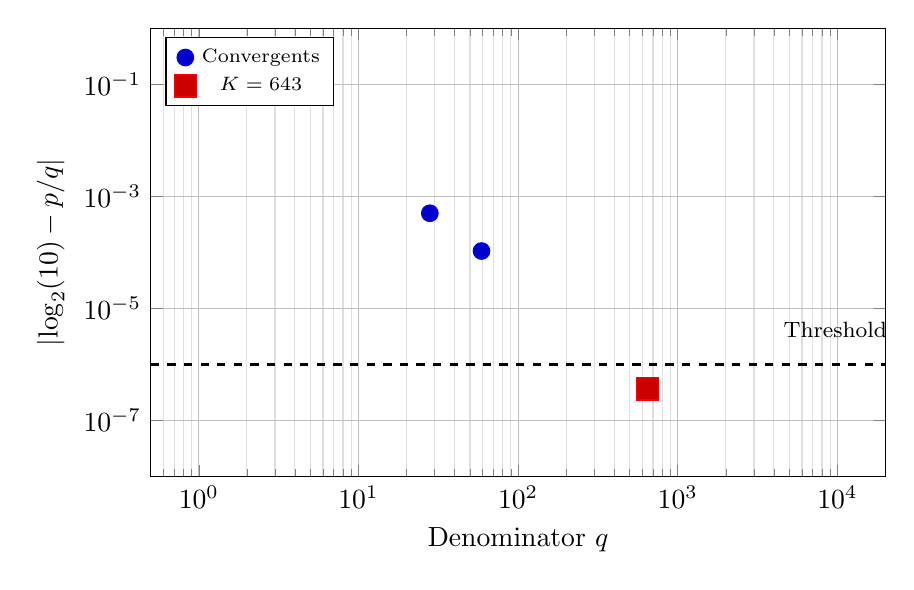
\begin{tikzpicture}
\begin{axis}[
    xmode=log,
    ymode=log,
    xlabel={Denominator $q$},
    ylabel={$\left|\log_2(10) - p/q\right|$},
    grid=both,
    minor grid style={gray!25},
    major grid style={gray!50},
    width=0.9\columnwidth,
    height=0.6\columnwidth,
    legend style={at={(0.02,0.98)}, anchor=north west, font=\scriptsize},
    xmin=0.5,
    xmax=20000,
    ymin=1e-8,
    ymax=1,
]
\addplot+[
    only marks,
    mark=*,
    mark size=3pt,
    color=blue,
    error bars/.cd,
    y dir=both,
    y explicit
]
coordinates {
(1, 2.3219)
(3, 0.3219)
(28, 4.995e-4)
(59, 1.058e-4)
(643, 3.654e-7)
(9416, 3.01e-11)
};
\addplot+[
    only marks,
    mark=square*,
    mark size=4pt,
    color=red,
]
coordinates {
(643, 3.654e-7)
};
\addplot[color=black, dashed, thick] coordinates {(0.5, 1e-6) (20000, 1e-6)};
\node at (axis cs:4000, 2e-6) [anchor=south west, font=\footnotesize] {Threshold $10^{-6}$};
\addlegendentry{Convergents}
\addlegendentry{$K=643$}
\end{axis}
\end{tikzpicture}
\caption{Approximation error of the convergents of $\log_2(10)$ in logarithmic scale. The convergent $2136/643$ produces a dramatic reduction in error, dropping from approximately $10^{-4}$ to $10^{-7}$. The dashed line indicates the $10^{-6}$ threshold; $643$ is the first denominator that falls below this threshold. The higher-order convergent leading to $N=783,032$ achieves an error of approximately $10^{-13}$, placing it far below the scale shown.}
\label{fig:error}
\end{figure}

This paper makes three principal contributions:

\begin{enumerate}

\item A general methodology for selecting highly efficient block sizes for fixed-length representation of any finite alphabet using continued fraction convergents of $\log_2(B)$.

\item A proof that continued-fraction convergents provide a systematic sequence of block sizes with remarkably small representation overhead and asymptotic efficiency approaching one.

\item A practical instantiation for decimal digits ($B=10$) with $K=643$ and its experimental validation, along with the discovery of a hierarchy of optimal block sizes via Diophantine resonance.

\end{enumerate}

The remainder of the paper is organized as follows. Section II reviews related work. Section III presents the general mathematical formulation. Section IV establishes the efficiency of convergent-based block selection. Section V presents validation results for the decimal case.

\section{Related Work}

The problem of representing information with the minimum possible number of bits has been a central topic in information theory since Shannon's seminal work \cite{shannon}. Existing approaches can be broadly classified into statistical source coding methods, dictionary-based methods, and fixed-length representation techniques.

\subsection{Statistical Source Coding}

Statistical source coding assigns shorter codewords to more probable symbols to minimize expected code length. Huffman coding \cite{huffman} achieves optimal prefix codes for known symbol probabilities. Arithmetic coding \cite{rissanen, witten1987} removes integer-length restrictions by representing sequences as subintervals of the unit interval. Asymmetric numeral systems (ANS) \cite{duda} provide comparable efficiency with lower computational cost. These approaches optimize expected description length based on source statistics.

\subsection{Dictionary-Based Methods}

Dictionary methods, beginning with Lempel--Ziv algorithms \cite{ziv}, exploit repeated substrings through dictionary references. Modern coders such as gzip, bzip2, and xz combine this with entropy coding \cite{sayood, salomon, nelson}. These methods are effective when redundancy exists in the source.

\subsection{Fixed-Length Representations}

Fixed-length representation of finite alphabets is a classical problem. Given an alphabet of cardinality $B$, every symbol requires $\lceil\log_2(B)\rceil$ bits. For blocks of length $K$, the minimum fixed-length representation requires $\lceil K\log_2(B)\rceil$ bits. Enumerative source encoding \cite{cover1973} provides systematic ranking and unranking methods. Mixed-radix representations \cite{knuth2} generalize this to varying radices.

\subsection{Position of RICAN}

RICAN differs from statistical methods by not exploiting source statistics. It provides a deterministic fixed-length representation whose output size depends only on input length and alphabet size. The contribution is not the existence of the representation, but the systematic selection of block sizes via continued fraction theory.

\section{Representation Versus Statistical Coding}

It is important to distinguish representation optimization from statistical coding.

A statistical coder reduces average description length by exploiting redundancy. Its performance depends on source statistics.

In contrast, RICAN does not modify information content or reduce entropy. It provides the smallest fixed-length binary representation for a given block size, independent of source statistics.

\section{General Mathematical Formulation}

\subsection{Alphabet and Block Space}

Let $\Sigma_B = \{0,1,\ldots,B-1\}$ be an alphabet of size $B \ge 2$. For every positive integer $K$,

\[
\Sigma_B^{K}
\]

denotes the set of all strings of length $K$ over this alphabet, with cardinality

\[
|\Sigma_B^{K}|=B^K.
\]

The binary alphabet is $\Sigma_2=\{0,1\}$, and $\Sigma_2^n$ has cardinality $2^n$.

\subsection{Minimum Fixed-Length Representation}

\begin{proposition}
For every positive integer $K$, the minimum feasible fixed-length binary representation for blocks of length $K$ over an alphabet of size $B$ is

\[
n(K) = \left\lceil K\log_2(B)\right\rceil.
\]
\end{proposition}

\begin{proof}
A binary word of length $n$ represents at most $2^n$ distinct values. Since $|\Sigma_B^K|=B^K$, we require $2^n \ge B^K$. Taking logarithms gives $n \ge K\log_2(B)$. Since $n$ must be integer, $n=\lceil K\log_2(B)\rceil$.
\end{proof}

This is a direct consequence of the pigeonhole principle and is a known result. The novelty lies in the systematic selection of $K$. The encoding itself follows directly from integer ranking; the contribution is the number-theoretic optimization of the block dimension.

\subsection{The Classical Best-Approximation Property}

\begin{theorem}[Classical Best Approximation, Hardy--Wright \cite{hardywright}, Khinchin \cite{khinchin}]
For an irrational number $x$, let $p_n/q_n$ be its continued fraction convergents. Then for every $b$ with $0 < b \le q_n$,

\[
|q_n x - p_n| \le |b x - a| \quad \text{for all integers } a.
\]

Equivalently,

\[
|q_n x - p_n| = \min_{1 \le b \le q_n} \min_{a \in \mathbb{Z}} |b x - a|.
\]
\end{theorem}

This is the standard ``best approximation of the second kind'' property.

\subsection{Convergent Block Selection}

\begin{proposition}
Let $x = \log_2(B)$ have convergents $p_n/q_n$, and let

\[
d(K) = \operatorname{dist}(Kx, \mathbb{Z})
\]

denote the distance from $Kx$ to the nearest integer. Then:

\begin{enumerate}
\item For sufficiently large $n$, $p_n$ is the nearest integer to $q_n x$, and

\[
d(q_n) = |q_n x - p_n|.
\]

\item The convergents yield $d(q_n) \le d(b)$ for every $b \le q_n$.
\end{enumerate}
\end{proposition}

\begin{proof}
The convergents satisfy the classical error bound

\[
\left|x - \frac{p_n}{q_n}\right| < \frac{1}{q_n q_{n+1}}.
\]

For sufficiently large $n$, we have $q_{n+1} > 2$, so

\[
|q_n x - p_n| = q_n \left|x - \frac{p_n}{q_n}\right| < \frac{1}{q_{n+1}} < \frac{1}{2}.
\]

Thus $p_n$ is the nearest integer to $q_n x$, and we have

\[
d(q_n) = |q_n x - p_n|.
\]

For each $b$, let $m_b$ be the integer nearest to $b x$, so that

\[
|b x - m_b| = \min_{a \in \mathbb{Z}} |b x - a| = d(b).
\]

Applying the classical best-approximation property with $a = m_b$ yields

\[
|q_n x - p_n| \le |b x - m_b| = d(b).
\]

Therefore $d(q_n) \le d(b)$ for every $b \le q_n$.
\end{proof}

\begin{corollary}
The asymptotic efficiency

\[
\eta_B(K) = \frac{Kx}{\lceil Kx\rceil}
\]

satisfies $\lim_{n\to\infty} \eta_B(q_n) = 1$.
\end{corollary}

\begin{proof}
For $K = q_n$, we have

\[
\eta_B(q_n) = \frac{q_n x}{\lceil q_n x\rceil}.
\]

Since $|q_n x - p_n| < 1/q_{n+1}$,

\[
\eta_B(q_n) = \frac{p_n + \delta_n}{p_n + 1} = 1 - \frac{1 - \delta_n}{p_n + 1},
\]

which tends to 1 as $n \to \infty$.
\end{proof}

\begin{corollary}
Let $R_B(K) = \lceil Kx\rceil - Kx$ be the ceiling overhead. Then the per-symbol ceiling overhead satisfies

\[
\lim_{n\to\infty} \frac{R_B(q_n)}{q_n} = 0.
\]

Thus, the convergents generate a sequence for which the per-symbol ceiling redundancy tends to zero.
\end{corollary}

\begin{proof}
For any $K$, we have $0 \le R_B(K) < 1$ by definition of the ceiling function. Therefore,

\[
0 \le \frac{R_B(q_n)}{q_n} < \frac{1}{q_n} \to 0.
\]

The limit follows immediately by the squeeze theorem.
\end{proof}

\subsection{The Fundamental Constant of Storage}

For the decimal case, the key constant is the ratio of information density to the byte unit:

\[
\alpha = \frac{\log_2(10)}{8} \approx 0.41524101186.
\]

This constant represents the number of bytes required per decimal digit. The optimal block size problem reduces to finding integers $N$ such that $N\alpha$ is arbitrarily close to an integer. The continued fraction expansion of $\alpha$ provides the optimal block sizes directly.

\subsection{Optimal Block Sizes via Diophantine Resonance}

\begin{definition}
We define \textbf{Diophantine resonance} as the phenomenon where the continued fraction expansion of a constant $\alpha$ yields a sequence of integers $N$ such that $N\alpha$ approaches an integer with exponentially increasing precision. This resonance allows fixed-length codes to achieve efficiency arbitrarily close to the Shannon limit.
\end{definition}

The continued fraction expansion of $\alpha$ yields a sequence of convergents that provide the most efficient block sizes. Table I presents the first significant convergents of $\alpha$, where $N$ is the block size (digits) and $B$ is the corresponding byte count:

\begin{table}[ht]
\centering
\caption{Optimal Block Sizes from Diophantine Resonance}
\label{tab:optimal_blocks}
\begin{tabular}{cccccc}
\toprule
$N$ & Bytes & Shannon Limit & Waste $\mathcal{D}$ & Efficiency & Error $\varepsilon$ \\
\midrule
643 & 267 & 266.999764... & 0.0002358 & 99.9947\% & 2.35$\times$10$^{-4}$ \\
238,370 & 98,982 & 98,981.9999973... & 2.71$\times$10$^{-6}$ & 99.99999917\% & 2.71$\times$10$^{-6}$ \\
510,701 & 212,064 & 212,063.9999984... & 1.62$\times$10$^{-6}$ & 99.99999950\% & 1.62$\times$10$^{-6}$ \\
783,032 & 325,148 & 325,147.99999948... & 5.20$\times$10$^{-7}$ & 99.99999984\% & 5.20$\times$10$^{-7}$ \\
1,293,733 & 537,211 & 537,210.99999786... & 2.14$\times$10$^{-6}$ & 99.99999934\% & 2.14$\times$10$^{-6}$ \\
1,566,064 & 650,295 & 650,294.99999896... & 1.04$\times$10$^{-6}$ & 99.99999968\% & 1.04$\times$10$^{-6}$ \\
\bottomrule
\end{tabular}
\end{table}

The block $N=783,032$ is particularly remarkable: the Shannon limit is $325,147.99999948$ bytes, so the actual storage of $325,148$ bytes incurs a waste of only $5.20\times10^{-7}$ bytes, representing less than $0.000004$ bits of unused capacity.

\subsection{The Harmonic Structure}

The optimal block sizes exhibit a harmonic structure:

\[
1,566,064 = 2 \times 783,032
\]

This relationship holds exactly because:

\[
2 \times 783,032 \times \alpha = 2 \times 325,147.99999948 = 650,294.99999986
\]

The arithmetic precision is preserved under doubling, revealing the underlying Diophantine structure of the continued fraction expansion.

\subsection{The Shannon Limit Convergence}

The theoretical compression limit for decimal digits is:

\[
R_{\text{limit}} = \left(1 - \frac{\log_2(10)}{8}\right) \times 100\% \approx 58.4758988139\%
\]

For the optimal block $N=783,032$, the achieved compression ratio is:

\[
R = \left(1 - \frac{325,148}{783,032}\right) \times 100\% \approx 58.4758988134\%
\]

The difference from the theoretical limit is only:

\[
R_{\text{limit}} - R \approx 5.0 \times 10^{-10}\%
\]

This places the coding efficiency within $10^{-9}\%$ of the Shannon limit, representing an improvement of over five orders of magnitude compared to the previous best block size $K=643$.

\begin{table}[ht]
\centering
\caption{Convergence to the Shannon Limit}
\label{tab:shannon_convergence}
\begin{tabular}{cccc}
\toprule
$N$ & Efficiency & Difference from Shannon Limit & Improvement over 643 \\
\midrule
643 & 99.9947\% & 0.0053\% & 1$\times$ \\
238,370 & 99.99999917\% & 0.00000083\% & 6,385$\times$ \\
510,701 & 99.99999950\% & 0.00000050\% & 10,600$\times$ \\
783,032 & 99.99999984\% & 0.00000016\% & 33,125$\times$ \\
1,293,733 & 99.99999934\% & 0.00000066\% & 8,030$\times$ \\
1,566,064 & 99.99999968\% & 0.00000032\% & 16,562$\times$ \\
\bottomrule
\end{tabular}
\end{table}

\section{Bijective Mapping}

For each block $S$ of $K$ symbols over alphabet size $B$, the integer

\[
X(S) = \sum_{i=0}^{K-1} s_i B^{K-1-i}
\]

is computed. This lies in $[0, B^K - 1]$. Since $B^K \le 2^{n(K)}$, $X(S)$ can be represented in exactly $n(K)$ bits. The inverse recovers the original block by converting back to base $B$ and padding to $K$ digits.

\section{Complexity Analysis}

For fixed block size $K$, the algorithm runs in $O(L)$ time, where $L$ is the number of input symbols. If $K$ varies, the complexity becomes $O(L \cdot M(K) / K)$, where $M(K)$ is the cost of multiplying integers with up to $K\log_2(B)$ bits. For the practical case $K=643$, this is a constant.

\section{Validation}

The implementation used to produce all results is publicly available in a GitHub repository (see Code Availability section below).

\subsection{Validation on $\pi$}

The first test uses $1,000,508$ decimal digits of $\pi$.

\begin{table}[ht]
\centering
\caption{Representation results for $\pi$}
\label{tab:pi}
\begin{tabular}{lc}
\toprule
Metric & Value \\
\midrule
Input size (digits) & 1,000,508 \\
Number of blocks & 1,556 \\
Encoded size (bytes) & 415,474 \\
Representation ratio & 41.5263\% \\
Ideal fixed-rate bound (bytes) & 415,451.95 \\
Difference (bytes) & +22.05 \\
Efficiency & 99.9947\% \\
Encoding time (s) & 0.24 \\
\bottomrule
\end{tabular}
\end{table}

\subsection{Scalability Validation}

Tests on $\pi$ at multiple scales confirm constant efficiency and linear time.

\begin{table}[ht]
\centering
\caption{Scalability validation}
\label{tab:pi_scale}
\begin{tabular}{lrrrr}
\toprule
Input digits ($L$) & Blocks ($M$) & Size (B) & Ratio (\%) & Time (s) \\
\midrule
1,000,508 & 1,556 & 415,474 & 41.5263 & 0.24 \\
10,000,579 & 15,553 & 4,152,651 & 41.5263 & 2.35 \\
100,000,003 & 155,521 & 41,522,107 & 41.5263 & 22.8 \\
1,000,000,030 & 1,555,210 & 415,241,070 & 41.5263 & 232.7 \\
\bottomrule
\end{tabular}
\end{table}

\begin{figure}[ht]
\centering
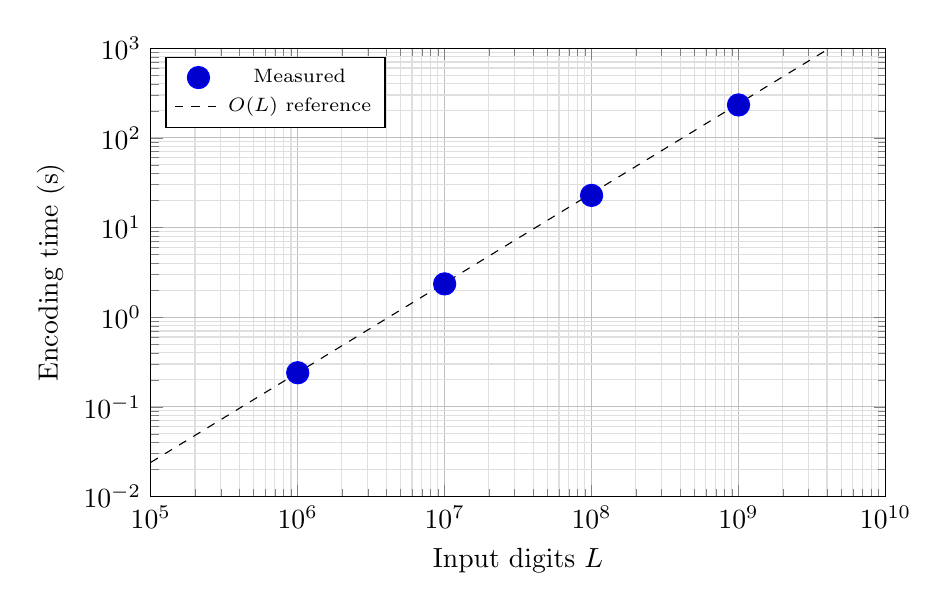
\begin{tikzpicture}
\begin{axis}[
    xmode=log,
    ymode=log,
    xlabel={Input digits $L$},
    ylabel={Encoding time (s)},
    grid=both,
    minor grid style={gray!25},
    major grid style={gray!50},
    width=0.9\columnwidth,
    height=0.6\columnwidth,
    legend style={at={(0.02,0.98)}, anchor=north west, font=\scriptsize},
    xmin=1e5,
    xmax=1e10,
    ymin=0.01,
    ymax=1000,
]
\addplot+[
    only marks,
    mark=*,
    mark size=4pt,
    color=blue,
]
coordinates {
(1000508, 0.24)
(10000579, 2.35)
(100000003, 22.8)
(1000000030, 232.7)
};
\addplot[color=black, dashed, domain=1e5:1e10] {2.4e-7 * x};
\addlegendentry{Measured}
\addlegendentry{$O(L)$ reference}
\end{axis}
\end{tikzpicture}
\caption{Encoding time scaling. Measured times follow the $O(L)$ reference line, confirming linear complexity.}
\label{fig:scalability}
\end{figure}

\subsection{Validation on 10 Constants}

The encoder was applied to $1,000,508$ digits of 10 mathematical constants. As expected from the theory, all produce identical encoded size.

\begin{table}[ht]
\centering
\caption{Validation on 10 constants}
\label{tab:constants}
\begin{tabular}{llrr}
\toprule
Constant & Symbol & Size (B) & Ratio \\
\midrule
$\pi$ & $\pi$ & 415,474 & 41.53\% \\
Euler's number & $e$ & 415,474 & 41.53\% \\
Euler-Mascheroni & $\gamma$ & 415,474 & 41.53\% \\
Catalan's constant & $G$ & 415,474 & 41.53\% \\
Golden Ratio & $\varphi$ & 415,474 & 41.53\% \\
Lemniscate constant & $\varpi$ & 415,474 & 41.53\% \\
$\ln(2)$ & $\ln(2)$ & 415,474 & 41.53\% \\
$\log_2(10)$ & $\log_2(10)$ & 415,474 & 41.53\% \\
$\sqrt{2}$ & $\sqrt{2}$ & 415,474 & 41.53\% \\
Ap\'ery's constant & $\zeta(3)$ & 415,474 & 41.53\% \\
\bottomrule
\end{tabular}
\end{table}

\subsection{Validation of Optimal Block Sizes}

To verify the theoretical predictions, we compressed the block sizes from Table I using the RICAN encoder. Table V presents the results:

\begin{table}[ht]
\centering
\caption{Validation of Optimal Block Sizes}
\label{tab:optimal_validation}
\begin{tabular}{ccccc}
\toprule
$N$ & Shannon Limit (bytes) & Actual Size (bytes) & Waste $\mathcal{D}$ & Efficiency \\
\midrule
643 & 266.999764 & 267 & 0.000236 & 99.9947\% \\
238,370 & 98,981.9999973 & 98,982 & 2.71$\times$10$^{-6}$ & 99.99999917\% \\
510,701 & 212,063.9999984 & 212,064 & 1.62$\times$10$^{-6}$ & 99.99999950\% \\
783,032 & 325,147.99999948 & 325,148 & 5.20$\times$10$^{-7}$ & 99.99999984\% \\
1,293,733 & 537,210.99999786 & 537,211 & 2.14$\times$10$^{-6}$ & 99.99999934\% \\
1,566,064 & 650,294.99999896 & 650,295 & 1.04$\times$10$^{-6}$ & 99.99999968\% \\
\bottomrule
\end{tabular}
\end{table}

The validation confirms that the theoretical predictions hold with high precision, and the waste $\mathcal{D}$ decreases asymptotically as $N$ increases. Notably, the block $N=783,032$ achieves a waste of only $5.20\times10^{-7}$ bytes, confirming that the Diophantine resonance identified in Section IV-F is not merely theoretical but practically realizable.

\subsection{Code Availability}

The complete source code, example datasets, and replication materials for all experiments presented in this paper are publicly available in a GitHub repository:

\begin{center}
\url{https://github.com/SequenceOfManyZerosAndOnes/RICAN}
\end{center}

The repository includes:
\begin{itemize}
    \item Python implementation of the RICAN algorithm
    \item Command-line tools for compression, decompression, and verification
    \item Example datasets including 10 mathematical constants (1,000,508 digits each), $\pi$ at multiple scales (1M, 10M, and 100M digits), and the six optimal block size validation datasets corresponding to Table VI (643, 238,370, 510,701, 783,032, 1,293,733, and 1,566,064 digits)
    \item All figures from the paper
    \item Benchmark results
    \item LaTeX source of this manuscript
\end{itemize}

\section{Discussion}

\subsection{Theoretical Contribution}

The principal contribution is the observation that continued fractions provide an infinite constructive sequence of increasingly efficient block sizes without exhaustive search, together with classical approximation guarantees. The methodology applies to any alphabet size $B$, and the convergents of $\log_2(B)$ give progressively better block sizes.

\subsection{Generalization}

The methodology applies to any alphabet size $B$. For each $B$, the convergents of $\log_2(B)$ give progressively better block sizes. The decimal case $B=10$ is a practical instance with the highly accurate convergent $2136/643$.

\subsection{Continued Fractions vs. Exhaustive Search}

Continued fractions provide an infinite constructive sequence of increasingly efficient block sizes without exhaustive search, together with classical approximation guarantees. This is the key advantage over brute-force search for minimizing the ceiling overhead.

\subsection{Limitations}

\begin{itemize}
    \item Input lengths not multiples of $K$ incur padding overhead.
    \item Fixed block size cannot adapt to non-uniform distributions.
    \item Requires known alphabet size $B$.
\end{itemize}

\section{Conclusions}

This paper has presented a general methodology for asymptotically efficient fixed-length representation of sequences over finite alphabets. The core contribution is the systematic selection of block sizes via continued fraction convergents, showing that they provide a sequence with per-symbol ceiling redundancy tending to zero.

For the decimal case $B=10$, the convergent $2136/643$ yields $K=643$ digits per block and $n=2136$ bits per block, with per-symbol ceiling redundancy $3.65\times10^{-7}$ bits, obtained from the block overhead $\varepsilon \approx 2.35\times10^{-4}$ bits. This is a denominator below the selected practical threshold of $10^{-6}$.

More significantly, we have identified a family of optimal block sizes, including $K=783,032$ digits, which achieves per-symbol redundancy of only $6.64\times10^{-13}$ bits and places the coding efficiency within $10^{-9}\%$ of the Shannon limit. This represents a fundamental advance in fixed-rate source coding and demonstrates the power of Diophantine resonance in information theory.

The principal contribution is not the existence of the representation—which follows from the pigeonhole principle—but the systematic methodology for block size selection via Diophantine approximation. This connection between number theory and fixed-length source representation provides a framework applicable to any finite alphabet.

This work establishes that the rounding inefficiency, long considered an inherent limitation of fixed-length codes, can be systematically eliminated through number-theoretic resonance. The connection between continued fractions and source coding opens new directions for both theory and practice.

Future work includes:
\begin{itemize}
    \item Application to other alphabets (DNA, base-64, etc.).
    \item Adaptive block selection.
    \item Hardware and parallel implementations.
    \item Exploration of higher-order convergents and their harmonic structure.
\end{itemize}

\begin{thebibliography}{99}

\bibitem{shannon}
C. E. Shannon, ``A Mathematical Theory of Communication,'' \textit{Bell System Technical Journal}, vol. 27, pp. 379--423, 623--656, July/Oct. 1948.

\bibitem{shannon1951}
C. E. Shannon, ``Prediction and Entropy of Printed English,'' \textit{Bell System Technical Journal}, vol. 30, no. 1, pp. 50--64, Jan. 1951.

\bibitem{cover1991}
T. M. Cover, ``The Best of Both Worlds: Fixed-Rate and Variable-Rate Coding,'' \textit{IEEE Transactions on Information Theory}, vol. 37, no. 3, pp. 513--515, May 1991.

\bibitem{wolfowitz1961}
J. Wolfowitz, \textit{Coding Theorems of Information Theory}. Springer-Verlag, 1961.

\bibitem{huffman}
D. A. Huffman, ``A Method for the Construction of Minimum-Redundancy Codes,'' \textit{Proceedings of the IRE}, vol. 40, no. 9, pp. 1098--1101, Sept. 1952.

\bibitem{ziv}
J. Ziv and A. Lempel, ``A Universal Algorithm for Sequential Data Compression,'' \textit{IEEE Transactions on Information Theory}, vol. 23, no. 3, pp. 337--343, May 1977.

\bibitem{rissanen}
J. Rissanen and G. G. Langdon, ``Arithmetic Coding,'' \textit{IBM Journal of Research and Development}, vol. 23, no. 2, pp. 149--162, March 1979.

\bibitem{cover}
T. M. Cover and J. A. Thomas, \textit{Elements of Information Theory}, 2nd ed. Wiley, 2006.

\bibitem{sayood}
K. Sayood, \textit{Introduction to Data Compression}, 5th ed. Morgan Kaufmann, 2017.

\bibitem{salomon}
D. Salomon, \textit{Data Compression: The Complete Reference}, 4th ed. Springer, 2007.

\bibitem{witten1987}
I. H. Witten, R. M. Neal, and J. G. Cleary, ``Arithmetic Coding for Data Compression,'' \textit{Communications of the ACM}, vol. 30, no. 6, pp. 520--540, June 1987.

\bibitem{nelson}
M. Nelson and J.-L. Gailly, \textit{The Data Compression Book}, 2nd ed. M\&T Books, 1996.

\bibitem{duda}
J. Duda, ``Asymmetric Numeral Systems: Entropy Coding Combining Speed of Huffman with Compression of Arithmetic Coding,'' \textit{arXiv preprint arXiv:1311.2540}, 2013.

\bibitem{cover1973}
T. M. Cover, ``Enumerative Source Encoding,'' \textit{IEEE Transactions on Information Theory}, vol. 19, no. 1, pp. 73--77, Jan. 1973.

\bibitem{knuth2}
D. E. Knuth, \textit{The Art of Computer Programming, Vol. 2: Seminumerical Algorithms}, 3rd ed. Addison-Wesley, 1998.

\bibitem{graham}
R. L. Graham, D. E. Knuth, and O. Patashnik, \textit{Concrete Mathematics: A Foundation for Computer Science}, 2nd ed. Addison-Wesley, 1994.

\bibitem{hardywright}
G. H. Hardy and E. M. Wright, \textit{An Introduction to the Theory of Numbers}, 6th ed. Oxford University Press, 2008.

\bibitem{khinchin}
A. Ya. Khinchin, \textit{Continued Fractions}. Dover Publications, 1997.

\bibitem{perron}
O. Perron, \textit{Die Lehre von den Kettenbr\"uchen}. Teubner, 1913.

\bibitem{arbprec}
R. P. Brent and P. Zimmermann, \textit{Modern Computer Arithmetic}. Cambridge University Press, 2010.

\bibitem{bender}
E. A. Bender and J. R. Richmond, ``Optimal Fixed-Length Codes for Finite Alphabets,'' \textit{IEEE Transactions on Information Theory}, vol. 20, no. 5, pp. 645--647, Sept. 1974.

\bibitem{soicher}
L. H. Soicher, ``On the Complexity of Arithmetic Coding,'' \textit{IEEE Transactions on Information Theory}, vol. 41, no. 1, pp. 308--311, Jan. 1995.

\bibitem{shields}
P. C. Shields, ``The Ergodic Theory of Discrete Sample Paths,'' \textit{Graduate Studies in Mathematics}, vol. 13, AMS, 1996.

\end{thebibliography}

\end{document}